\section{Performance Evaluation}
\label{sec:PerformanceEvaluation}
\subsection{Simulation}
We first use simulation data to demonstrate the effectiveness of our cluster-based modal analysis approach and the clustering algorithms. We fix all associated parameters except two: the network topology and the transmission power \(e_T\). Although in some circumstances, these two factors are correlated, they are independently considered in this simulation. A total of 40 sensor nodes are randomly deployed starting from a relatively sparse wireless sensor network with network degree, defined using the node with the minimum degree in the network, is 3. Under this network degree, we considered energy consumptions when the transmission power \(e_T\) is changing from \(5e-4\) to \(2.5e-3\), with the interval of \(5e-4\).  The energy consumption of the following four approaches are considered:(1) the traditional approach when all the raw data are streamed back to a sink node, (2) the cluster-based modal analysis with clusters generated from the \(1^{st}\) centralized algorithm, (3) from the \(2^{nd}\) centralized algorithm and (4) from the distributed algorithm. In the first approach, the sink node is chosen to be the node whose short path tree (SPT) is the shortest among all the other nodes. Also, no computation energy is included in this approach. A total of 500 simulations are performed and the average energy consumption of each approach is calculated. The above procedure is repeated when the network degree is changed to be 4 and 5.

The parameters associated with the simulation are listed in Table \ref{tab:Table2} and the simulation results are shown in Fig. \ref{fig:Simulation2}. It can be seen that for the first traditional approach, the total energy is linearly increased with the increase of \(e_T\) and the slope is the length of the SPT rooted at the sink node.  The cluster-based approach, either using clusters generated from centralized or distributed algorithms, is much more energy efficient compared with the traditional approach. This conclusion is more evident when the transmission power \(e_T\) is large. When \(e_T = 2.5e-3\), the energy consumption of the cluster-based approach is about one fifth of the traditional approach.  For the cluster-based approach, it seems that using clusters generated from the \(1^{st}\) centralized algorithm and from the distributed algorithm are slightly better than the \(2^{nd}\) centralized algorithm. 

\begin{figure}
	\centering
		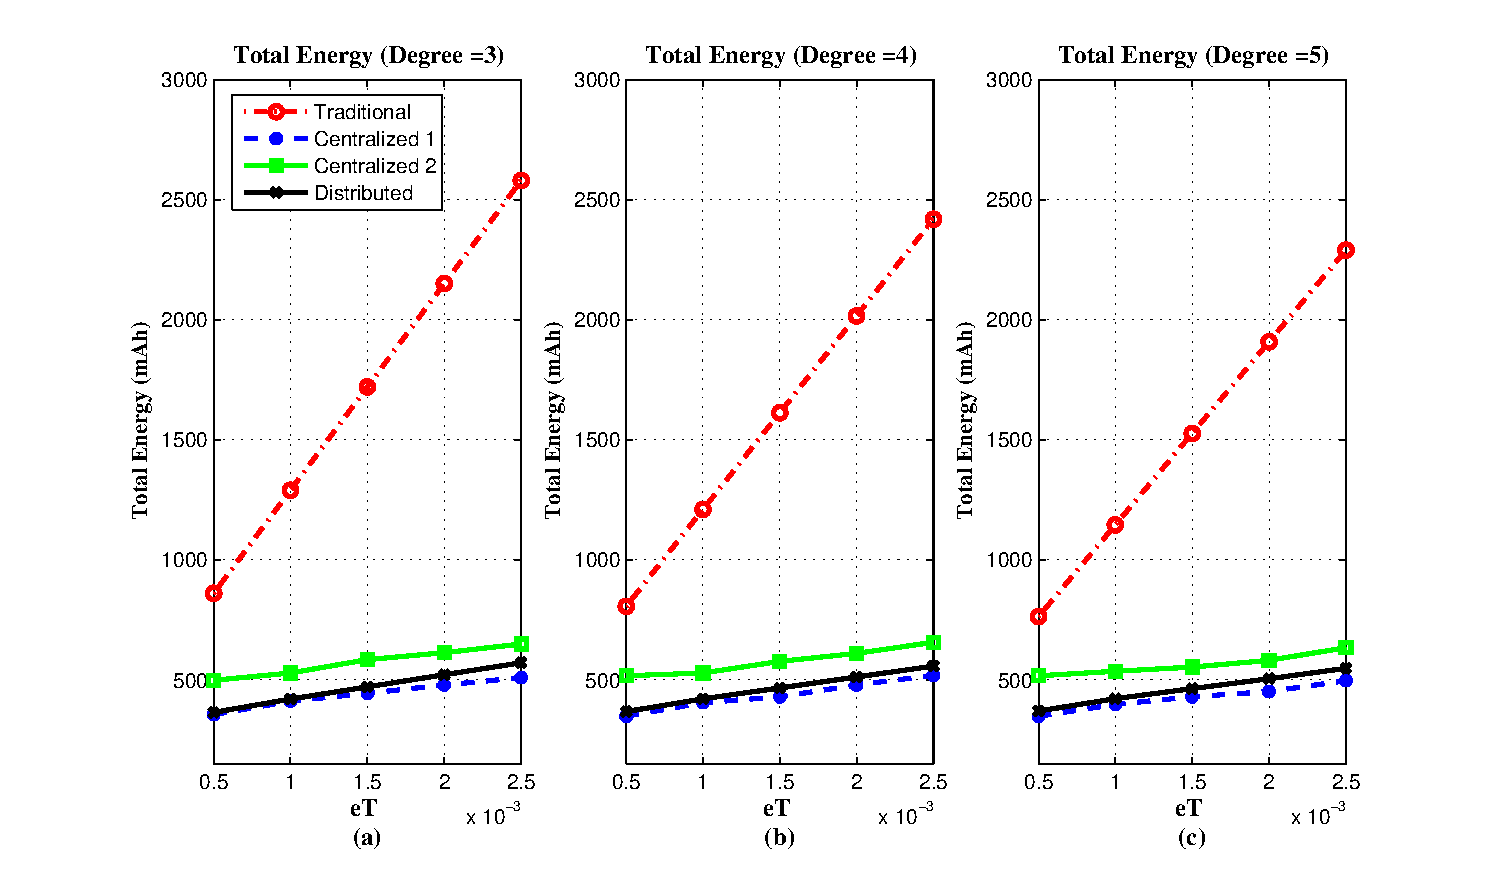
\includegraphics[width=.40\textwidth,height=.25\textwidth]{Simulation2.eps}
	\caption{The total energy in different scenarios. (a)Network Degree=3 (b)Network Degree=4 (c) Network Degree=5}
	\label{fig:Simulation2}
\end{figure}

To further demonstrate the importance of using optimal cluster size, we illustrate in Fig. 
\ref{fig:SimOptNumber} the energy consumption when the \(1^{st}\) algorithm chooses three different cluster sizes: \(n_{opt}-1\), \(n_{opt}\) and \(n_{opt}+1\). It can be seen that compared with other cluster sizes, clustering using designed optimal cluster size can achieve lower energy consumption. 

\begin{figure}
	\centering
		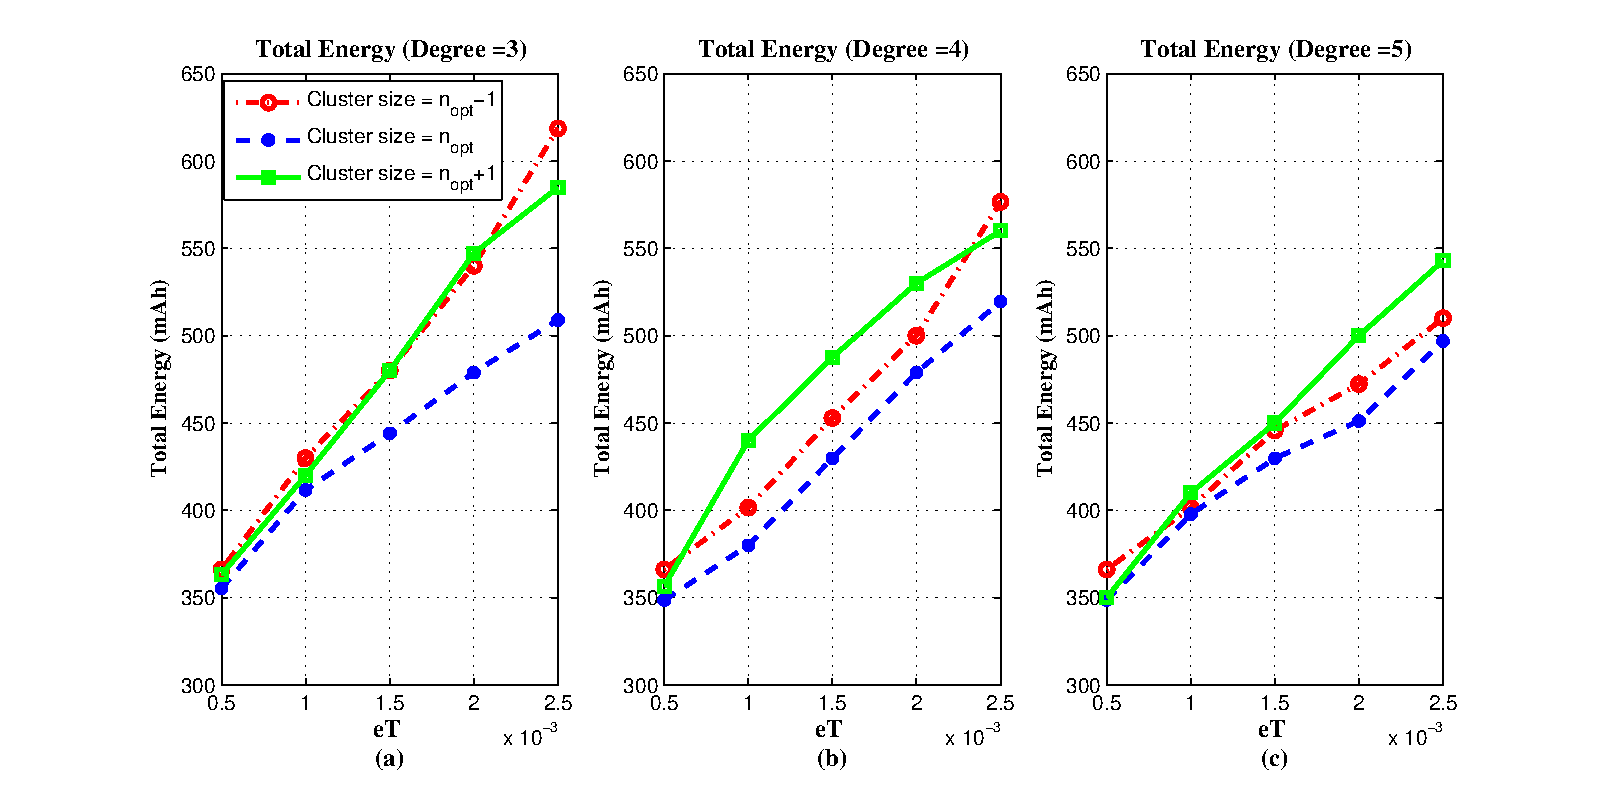
\includegraphics[width=.49\textwidth,height=.25\textwidth]{SimOptNumber.eps}
	\caption{The energy consumption using different cluster sizes. (a)Network Degree=3 (b)Network Degree=4 (c) Network Degree=5}
	\label{fig:SimOptNumber}
\end{figure}

\subsection{Implementation}
We have tested our cluster-based modal analysis approach through a real implementation. The wireless sensor nodes adopted are called SHM Mote and are particularly developed for general SHM applications (see Fig.\ref{fig:SHMMote}). A SHM Mote includes an Intel Imote2, a sensor board, an external 32Mb non-volatile memory chip, an AM radio receiver for synchronized sensing, and a RF amplifier. 

\begin{figure}
\centering
\subfloat[SHM Mote]{\label{fig:SHMMote}
%\figurecurrentwidth{originalbeam}}
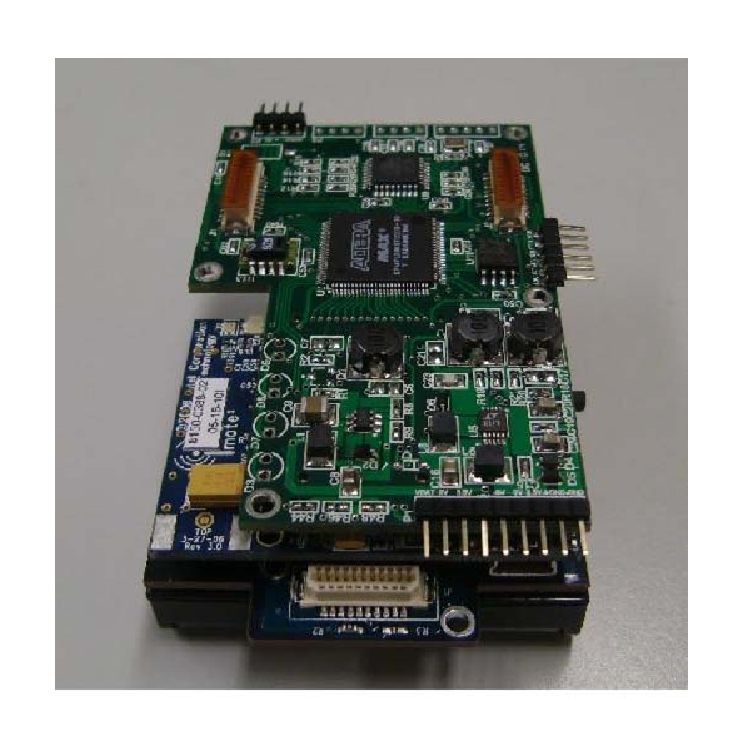
\includegraphics[width=.15\textwidth, height=0.2\textwidth]{SHMMote.eps}}
%\qquad
\subfloat[Testing structure]{\label{fig:TestStructure}
%\figurecurrentwidth{mode1}}
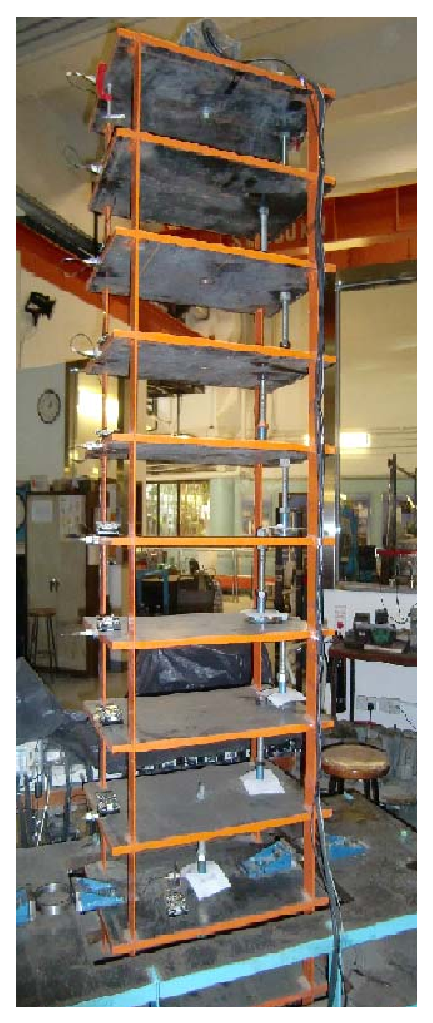
\includegraphics[width=.15\textwidth, height=0.3\textwidth]{TestStructure.eps}}
\subfloat[Network topology]{\label{fig:Testbedtopology}
%\figurecurrentwidth{originalbeam}}
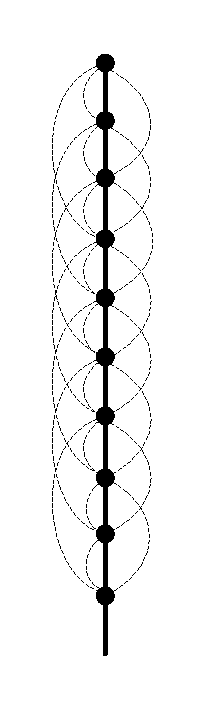
\includegraphics[width=.11\textwidth, height=0.32\textwidth]{Testbedtopology.eps}}
\caption{SHM Mote and testing structure}
\label{fig:SHMMOTEandTestStructure}
\end{figure}

Fig. \ref{fig:SHMMote} shows the setting of the lab test. The test building has 10 floors, at each floor, a Mote is deployed to monitor the structure's horizontal accelerations. We adjust the transmission power to be \(e_T =1e-5\) in this test after a few tests on link-quality. Under this transmission power, the topology of the network along with the simplified structure are illustrated in Fig. \ref{fig:TestStructure}. We use a gateway node which is connected a computer for the control purpose, while this gateway can be removed in future implementation. The SHM Motes run modified TinyOS and are configured to sample the accelerometers in a synchronized manner at frequency of 512Hz. Under the command of gateway, each Mote starts collecting \(N = 10752\) data samples synchronously.  The cluster information is calculated by the \(1^{st}\) centralized algorithm run in the computer and then is feed to each node through wireless link. In this implementation, the optimal cluster size is \(n_{opt}=7\) and these ten sensor nodes are partitioned into 2 clusters as illustrated in Fig. \ref{fig:Testbedtopology}. Once each node has this information, the cluster-based modal analysis is implemented in each cluster, one cluster at a time, to identify the first three mode shapes of the structure.  The obtained mode shapes of each cluster are then transmitted back to the gateway and are assembled.  For comparison, traditional approach is also used in which all measured data are transmitted the gateway where the ERA using all the measurement data to identify the mode shapes of the whole structure.

Fig. \ref{fig:TestResults} illustrates the identified mode shapes by the traditional centralized modal analysis and by our cluster-based modal analysis. It can be seen that using cluster-based modal analysis, the mode shapes can be identified without losing much of the accuracy. Moreover, we tested that the energy communication cost is decreased from \(259mAh\) to \(152mAh\). 

\begin{figure}
\centering
\subfloat[Clustering using algorithm1]{\label{fig:Testbedcluster}
%\figurecurrentwidth{originalbeam}}
\includegraphics[width=.11\textwidth, height=0.32\textwidth]{Testbedclustering.eps}}
\subfloat[Mode shapes]{\label{fig:TestResults}
%\figurecurrentwidth{originalbeam}}
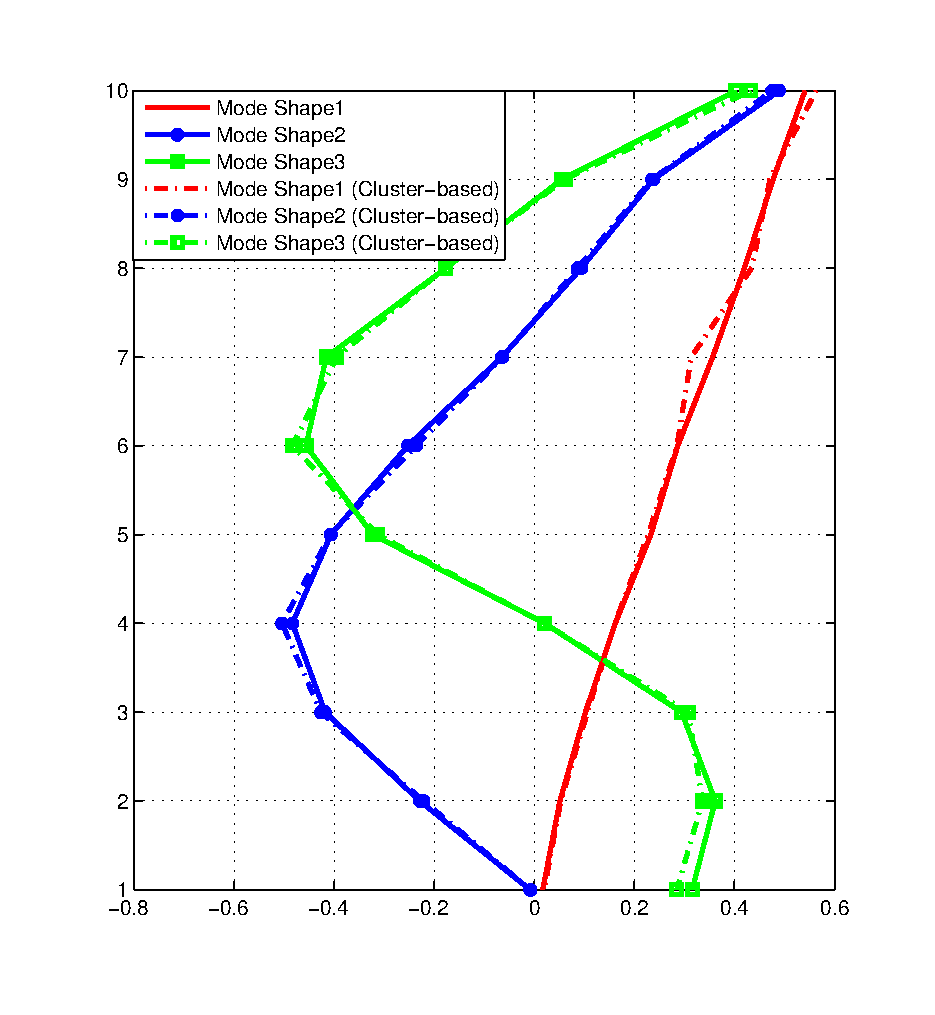
\includegraphics[width=.21\textwidth, height=0.32\textwidth]{TestResults.eps}}
\caption{Clustering and obtained mode shapes}
\label{fig:Clusteringwithmodeshapes}
\end{figure}



